\chapter{Experimental Design} \label{ch:Exp_Design}

\section{Testing Considerations}

Before venturing further, we now summarize the goals of the UKF framework described previously, paying particular attention to unmanned aircraft system (UAS) operations. This ROS package was designed with the express intent of producing estimates of the position vector $\mathbf{p}$ and orientation quaternion $\mathbf{q}$ of a rotorcraft UAV in real time. Thus, the experiments testing the system's efficacy compare the filter's estimates of position and orientation to the ground truth as measured by Vicon. Vicon, like many commercially available motion capture systems, works by using a number of infrared cameras (usually 8--12) to track the positions of retroreflector balls in the cameras' field of view. Each camera illuminates the area with infrared light, which is in turn reflected by the retroreflector balls. Sets of these retroreflectors can be grouped together in software to represent rigid objects, thus allowing the system to track not only the position of an object, but its orientation as well.

\begin{figure}[t]
    \centering
    \begin{subfigure}[t]{0.5\textwidth}
        \centering
        \includegraphics[width=0.8\textwidth]{sensor_mount_top}
        \caption{Top view of sensor mount.}
    \end{subfigure}%
    ~ 
    \begin{subfigure}[t]{0.5\textwidth}
        \centering
        \includegraphics[width=0.8\textwidth]{sensor_mount_bottom}
        \caption{Bottom view of sensor mount.}
    \end{subfigure}
    \caption[3D-printed Sensor Mount]{The 3D-printed sensor mount. In (a), the Phidgets IMU is on the left and the mvBlueFOX camera is on the right. In (b), the linear braking handle and camera lens are visible.}
    \label{fig:sensor_mount}
\end{figure}

\begin{figure}
  \centering
    \includegraphics[width=\textwidth]{whole_cart}
  \caption[Mobile Test Stand]{The mobile test stand, fully assembled. The aluminum rail holds the sensor mount 1~meter above the floor and is marked with an adhesive metric ruler for measuring camera displacement during PTAM initialization.}
  \label{fig:whole_cart}
\end{figure}

\begin{figure}
  \centering
    \includegraphics[width=\textwidth]{cart_at_AI}
  \caption[Testing Environment]{The mobile test stand in the testing environment. The area shown is part of a larger motion capture facility. The floor is covered with rubber tiles, many of which bear April tags and QR codes for visual geometry.}
  \label{fig:cart_at_AI}
\end{figure}

\begin{figure}
  \centering
    \includegraphics[width=\textwidth]{sensor_mount_vicon}
  \caption[Sensor Mount Instrumented with Retroreflectors]{Close-up view of the sensor mount instrumented with Vicon infrared retroreflector balls.}
  \label{fig:sensor_mount_vicon}
\end{figure}

This system depends upon two sensors: a global-shutter monocular camera and an IMU. The IMU used in this experiment contains a 3-axis accelerometer and 3-axis gyroscope. To simulate both sensors moving through the scene in a manner reminiscent of hovering rotorcraft flight, a rolling test stand was constructed to carry the sensors safely throughout a large motion capture environment. Mounting the sensor suite on a large, steady, level platform allows for a high degree of control over the accelerations and angular velocities felt by the IMU, as well as the motion captured by the ventral camera. In order to validate the UKF framework's effectiveness under ideal conditions, a modern laptop computer containing an Intel i7 processor with 16~GB of RAM was used for all computations. The floor of the motion capture environment was strewn with a mixture of April tags and modified Quick Response\footnote{\url{https://en.wikipedia.org/wiki/QR_code}} (QR) codes in order to provide sufficient visual features for PTAM to track.

\section{Experimental Procedures}

Two experiments were designed to characterize the UKF framework's effectiveness in various regimes of motion. In the first experiment, the mobile test stand was moved in a rectangular ``box'' pattern at approximately constant speed, without rotation.

\begin{figure}
  \centering
    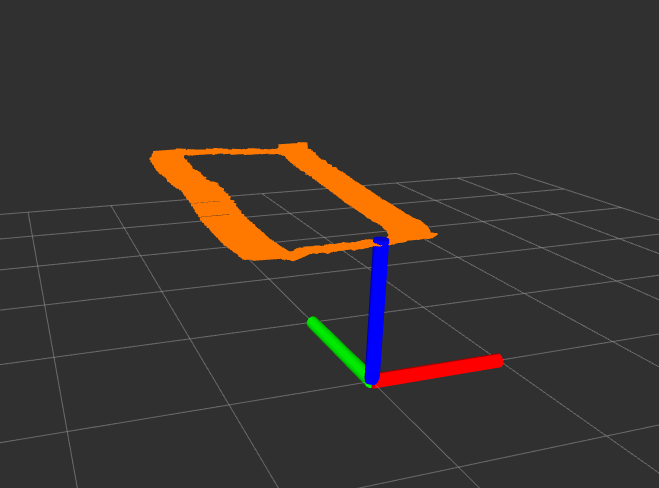
\includegraphics[width=\textwidth]{good_box_5_cropped}
  \caption[Rviz Visualization of a Box Pattern Trajectory]{An Rviz visualization of a box pattern trajectory. In this image, the orange segments are actually composed of arrows pointing along the vehicle's $x$-axis (parallel to the red axis at the origin). The experiment starts one meter above the origin and the cart is pushed in a rectangular pattern, coming to rest at the origin again.}
  \label{fig:good_box}
\end{figure}

\todo{describe each experiment}

Two data streams were collected for analysis using the \texttt{rosbag}\footnote{\url{http://wiki.ros.org/rosbag}} data recording utility.
\todo{more explanation of post processing}

\clearpage
\section{Materials}
\subsection{Computation and Sensing}
\begin{enumerate}
\item One (1) MatrixVision mvBlueFOX-MLC Camera\footnote{\url{https://www.matrix-vision.com/USB2.0-single-board-camera-mvbluefox-mlc.html}}
\item One (1) 1044\_0 PhidgetSpatial Precision 3/3/3 High Resolution IMU\footnote{\url{http://www.phidgets.com/products.php?product_id=1044}}
\item One (1) Hewlett-Packard Spectre x360 Convertible Laptop 13-ac076nr\footnote{\url{http://store.hp.com/us/en/pdp/hp-spectre-x360---13-ac076nr}}
\item Two (2) male Mini USB 2.0 to male USB Type A cables
\end{enumerate}
\subsection{Mobile Test Stand}
\begin{enumerate}
\item One (1) Oklahoma Sound PRC200 Premium Presentation Cart\footnote{\url{http://www.oklahomasound.com/products/product-category/single/?prod=9}}
\item One (1) 3D-printed Sensor Mount
\item Two (2) 4" C-Clamps
\item One (1) 1.2-meter 80/20\textsuperscript{\textregistered}~Inc.\ 1515 Rail\footnote{\url{https://8020.net/1515.html}}
\item One (1) 15 Series ``L'' Handle Linear Bearing Brake Kit\footnote{\url{https://8020.net/6800.html}}
\item One (1) $\frac{5}{16}$-18 $\times$ 0.687" Black FBHSCS (Screw)\footnote{\url{https://8020.net/shop/3320.html}}
\item Two (2) Slide-In Economy T-Nuts\footnote{Also available at \url{https://8020.net/shop/3320.html}}
\item Three (3) 1" Vicon Infrared Retroreflector Balls
\item Two (2) $\frac{1}{2}$" Vicon Infrared Retroreflector Balls
\item One (1) 0.7-meter Length of $\frac{1}{8}$"-thick Carbon Fiber Tube
\end{enumerate}
\pagebreak

\begin{figure}
  \centering
    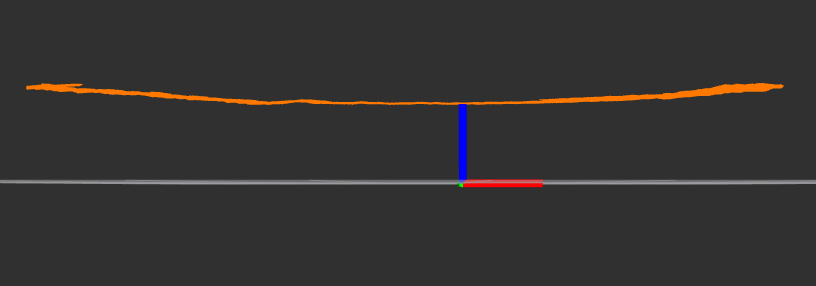
\includegraphics[width=\textwidth]{bowl-shaped_world}
  \caption[Rviz Visualization of Translational (Lens) Distortion]{An Rviz visualization of the ``bowl-shaped'' world seen by PTAM during a long translational motion. This image was created by translating the mobile test stand 3--4~meters in the $+x$ direction and then translating back 4--5~meters past the origin in the $-x$ direction.}
  \label{fig:bowl-shaped_world}
\end{figure}

\begin{figure}
  \centering
    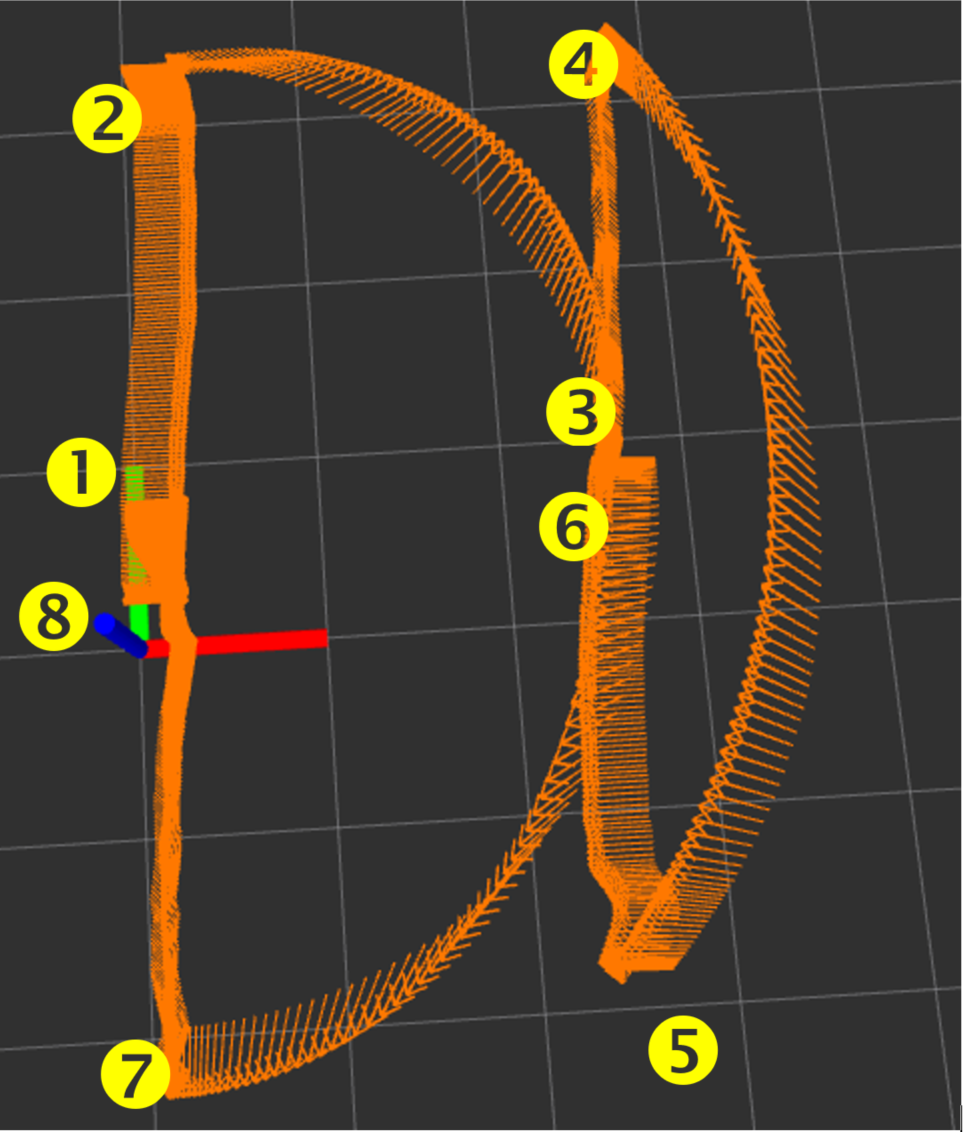
\includegraphics[height=0.8\textwidth]{rot_bug_rviz}
  \caption[Rviz Visualization of Rotational Distortion]{An Rviz visualization of aberrant rotational behavior. This image was created by moving the cart in a square (3~m~$\times$~3~m) pattern, making clockwise 90-degree turns at each corner.}
  \label{fig:rot_bug_rviz}
\end{figure}
\todo{write out explanation of figure}